\chapter{Background}
\label{ch:background}
In this chapter I am going to establish the foundation by giving a brief overview of LLMs, the CEFR framework and the challenges in language proficiency classification and text adaptation. I will also discuss existing solutions and their limitations. This chapter will provide the necessary background information to understand the research questions and methodology presented in the following chapters.

\section{Large Language Models}
\label{s:background_llms}
LLMs are a subset of machine learning models that leverage complex neural networks trained on vast amounts of text data to process and generate human-like text. Most newer and advanced models are based on the Transformer architecture \citep{Vaswani2017} which has shown remarkable capabilities in natural language processing tasks. Transformers are particularly well-suited for language modeling tasks due to its self-attention mechanism, which allows the model to focus on different parts of the input sequence when generating the output.

\begin{figure}[h]
    \centering
    \vspace{0.25cm}
    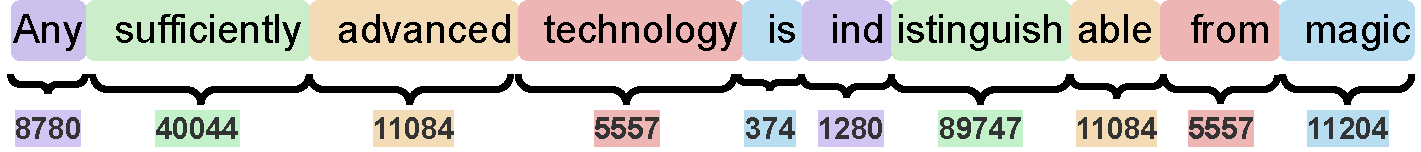
\includegraphics[width=0.98\textwidth]{img/tokenization.pdf}
    \caption{Example tokenization of a sentence for the LLaMA3 tokenizer \citep{LLamaTokenizerPlayground}}
    \label{fig:tokenization}
\end{figure}
This process begins with tokenization, where input text is divided into smaller units called tokens (see Figure \ref{fig:tokenization}).
% These tokens are then converted into numerical vectors (embeddings) that capture semantic meaning. Following that, they then get processed in the core of the transformer model: Multiple layers of self-attention and feed-forward neural networks. In self-attention layers, the model learns to identify relevant relationships between all tokens in the sequence. Subsequently, feed-forward layers further process this information and contain most of the models knowledge. The model then decodes this processed information to generate output text. Decoding happens token by token, with each new token being influenced by all previous tokens, until an end-of-sequence token is produced. As a result of this iterative process, the model can generate coherent and contextually relevant text.
Tokens are then transformed into numerical vectors (embeddings) that encapsulate semantic meaning. Subsequently, they are processed through the core of the transformer model: multiple layers of self-attention mechanisms and feed-forward neural networks. Within the self-attention layers, the model learns to identify and weigh relevant relationships between all tokens in the sequence. Following this, feed-forward layers further refine this information, effectively storing the model's knowledge. The model then decodes this processed information to generate output text. This decoding runs sequentially, with each new token being influenced by all preceding tokens, until an end-of-sequence token is produced. As a result of this iterative process, the model can generate coherent and contextually relevant text.

LLMs can be categorized into encoder-only (e.g. BERT \citep{Devlin2018}), decoder-only (e.g. GPT, LLaMA etc.. \citep{Brown2020,LLaMA3}) and encoder-decoder models (e.g. T5 \citep{Raffel2019}), each with its own strengths and weaknesses. Currently most advanced models are based on the decoder-only architecture. For a way more thorough explanation of LLMs and overview I recommend the reader to check out \cite{Zhao2023}.

LLMs have shown to be capable of generating coherent and contextually relevant text, making them suitable for a wide range of applications such as text generation, translation and summarization. But they have also some drawbacks and limitations: Due to their large size and complexity, they require significant computational resources during inference and training. Moreover, they are very sensitive to the quality and quantity of the training data, which can lead to bad quality responses or even worse, biased or harmful outputs.

\section{Fine-tuning}
\label{s:background_finetuning}
Fine-tuning is a technique for adapting a model trained on a broad, generalized dataset. It involves further training the model on a smaller, task-specific dataset, leveraging the model's general knowledge. Fine-tuning leads to small adjustments in the model's weights, which allows it to adapt to the specific task or domain resulting in improved performance. To make fine-tuning even more efficient, there are advanced techniques like low rank adaptation - often referred to as LoRa \citep{Hu2021}. It involves adding trainable rank decomposition matrices to the model's existing weights. This approach significantly reduces the number of trainable parameters, making fine-tuning more memory-efficient and faster, while still achieving comparable performance than traditional fine-tuning.

\section{Language Proficiency and CEFR}
\label{s:background_cefr}
Language proficiency describes the ability of an individual to use a language effectively and accurately in a variety of contexts and situations. The Common European Framework of Reference for Languages (CEFR) is a widely used framework that provides a standardized scale for assessing language proficiency. It divides language proficiency into six levels, ranging from A1 (beginner), A2 (elementary), B1 (intermediate), B2 (upper-intermediate), C1 (advanced) and C2 (proficient). The CEFR is used in language education and assessment to evaluate and certify language proficiency, and it provides a common reference point for language learners, teachers and institutions. There are rules and guidelines for each level, which describe the skills that learners should have at each level. For example, at the A1 level, learners should be able to understand and use familiar everyday expressions and basic phrases, while at the C2 level, learners should be able to understand complex texts and communicate fluently and spontaneously in a variety of contexts.
\section{Challenges in Language Proficiency Classification}
\label{s:background_challenges_classification}
Language proficiency classification is a challenging task, especially for traditional NLP techniques, due to the complexity and ambiguity of human language. There are no explicit rules that can be followed by a traditional algorithm to determine the proficiency level of a text, and the classification is often subjective and context-dependent. Moreover, the classification of language proficiency is not a binary decision, but rather a continuous scale, which makes it difficult to define clear boundaries between the different levels. This is further complicated by the fact that language proficiency is not only determined by the vocabulary and grammar used in a text, but also by the context, style and tone. For example, a text that uses simple vocabulary and grammar may still be classified as advanced if it discusses complex topics or uses sophisticated arguments. Traditional approaches to language proficiency classification rely on manual annotation and expert judgment, which are time-consuming and expensive. They also suffer from subjectivity and inconsistency, as different annotators may have different opinions on the proficiency level of a text. Here LLMs can provide a solution as they are designed to work with natural language text and have shown to be capable of understanding and working with the complexity and ambiguity of human language.
\section{Challenges in Text Transformation}
\label{s:background_challenges_transformation}
Text adaptation is the process of modifying a text to make it more suitable for a specific audience or purpose. In the context of language proficiency, text adaptation involves modifying a text to match the proficiency level of the reader. This can include simplifying the vocabulary and grammar, rephrasing complex sentences  and adding explanations or examples to make the text more understandable. Transferring is an even more challenging task than language proficiency classification, as it requires not only an understanding of the text itself, but also the ability to generate new text that is coherent and contextually relevant while matching the target proficiency level. Problems like this fit LLMs capabilities even more as they are designed to generate text and have shown to be capable of adapting text to different styles and contexts. Transformers are particularly well-suited for this task, as they were originally designed for translation between languages \citep{Vaswani2017} and translation of proficiency levels can be seen as a subset of that task.
\section{Existing Solutions and their Limitations}
\label{s:background_existing_solutions}
There are some approaches to CEFR classification of German texts. Notably there is the work of \cite{Szuuegyi2019}, \cite{Vajjala2018} and extending on that work, \cite{Caines2020}. These approaches all use traditional NLP techniques and machine learning algorithms to classify German (and other languages) texts according to the CEFR levels. They rely on linguistic features such as vocabulary, grammar and syntax to determine the proficiency level of a text. While these approaches have shown promising results, they have some limitations. They are often based on hand-crafted features and rules, which are time-consuming and expensive to create and maintain. Additionally due to their architecture and approach, these methods can not be used to adapt texts to different proficiency levels which is an integral part of this thesis.